
\chapter{Pariticle-In-Cell}
\label{chap:pic}

\section{等离子体数值模拟}
\begin{figure}[!htbp]
  \centering
  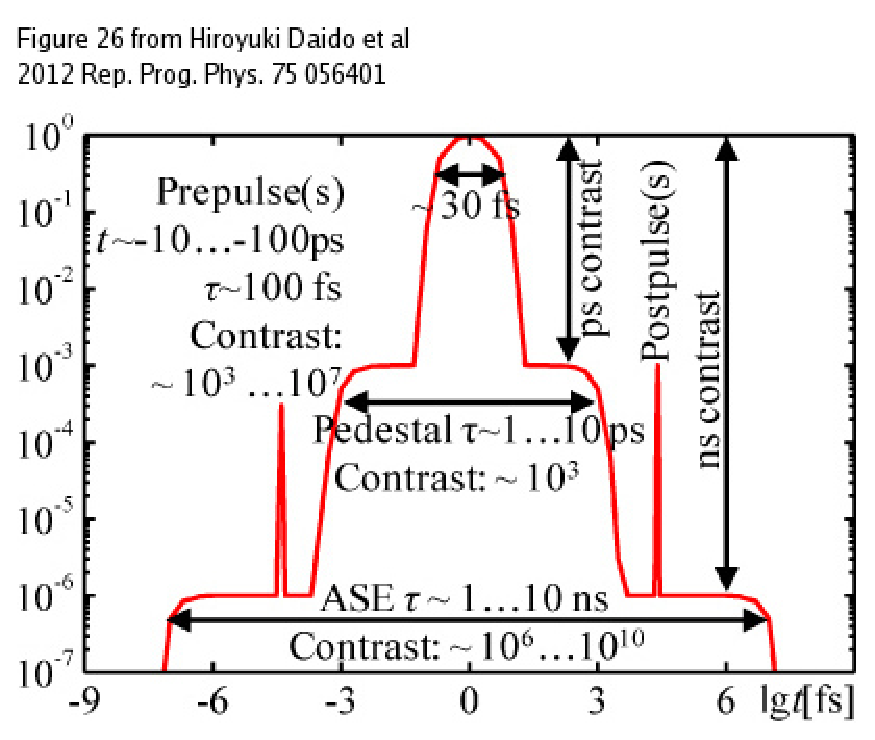
\includegraphics[width=\MyFactor\textwidth]{Img/prepulse2012.eps}
  \caption{激光脉冲示意图}
  \label{fig:prepulse2012}
\end{figure}

激光的相互过程中,设计到波-波、波-粒子、粒子-粒子的相互作
用,是一个多模、多粒子系统的强非线性相互作用过程。解析方法很难全面地进行研究,数值计算就是必然的选择。
数值模拟的方法在激光等离子体相互作用的领域中有重要的意义。首先,模拟工作往往具有前瞻性,许多重要的发现是建立在模拟工作的基础上,对实验提出要求与指导。由于数值模拟的灵活性,实验中难以达到的条件,可以在数值计算中进行模拟,寻找最优解决方法。同时,模拟工作可以解释实验中的新发现,全方位地对于物理过程进行剖析,有助于更好的理解实验现象。实验和模拟之间,互为依靠,相辅相承。现代数值模拟,借助与CPU以及GPU等高速计算工具,以及MPI和CUDA等优秀的计算平台,其计算功能已经相对成熟。
从模拟的算法角度,对于不同对象,模拟中采用不同的数值方法。对等离子体这种呈现集体运动特性的带电粒子的复杂系统(等离子体)的数值模拟研究,一般用流体力学模拟或动理学模拟方法


\subsection{流体力学模拟}


流体力学模拟方法从宏观角度研究等离子体特性,例如:温度、密度、压强等,其精度在空间上百微米量级,时间上纳秒量级。其方法,是将微观得到的吸收系数或输运系数的作为已知条件,求解磁流体力学(MHD)方程,得到粒子的分布统计信息。通过粒子分布函数对参量进行积分,得到统计意义上的结果。
完整的流体力学方程组,可以通过取 Vlasov 方程的不同的速度矩得到:

连续性方程:$\partial{n_j}/\partial{t}+\partial{n_j \bar{\vec{u_j}}}/\partial{t} =0$
运动方程:$n_j \partial {\vec{u_j}}/\partial{t}+n \vec{u_j} \partial{\vec{u_j}}/\partial{\vec{x}} = \frac{n_j q_j}{m_j} ( \vec{E}+\frac{\vec{u_j} \times \vec{B}}{c}) - \frac{1}{m_j} \frac{\partial{\vec{p_j}}}{\vec{x}}$

状态方程:

\[ \left\{
  \begin{array}{lr}
    p_j=n_j T_j & : $\omega / k ll v_j$\\
    \frac{p_j}{{n_j}^{\gamma}}=const & : $\omega / k gg v_j$
  \end{array}
\right.
\]

其中,j代表粒子种类,温度$T_j$,热速度 $v_j=(T_j/m_j)^{1/2}$,热压 $P_j$。
$\gamma=(2+N)/N$,N是自由度。加上maxwell方程,以上构成流体力学的完备描述。当 $\omega / k ll v_j$时,服从等温分布,当 $\omega / k gg v_j$时,服从绝热分布。当 $\omega / k = v_j$时,流体方法无法描述热传递过程,需要使用Vlasov方程。

\subsection{动力学模拟}


动理学模拟在微观上研究等离子体中的物理过程,考虑粒子在电磁场作用下运动。由于微观系统较大的复杂度,其研究等离子体的空间范围和时间尺度都有限,多用于微型空间中的快速过程。主要
包括两种方法:
(1) 求解动力学方程:
Vlasov 方程:
 
 
j 类 粒 子 在 相 空 间 ( x , v ) 中 的 配 置 随 时 间 变 化 的 函 数 f j ( x , v , t ) 满 足
 f j
q  1    f
  f
 v   j  j ( E  v  B )   j  0 ,它描述高温无碰撞等离子体,如受控热核
 t
 x m j
c
 v
反应和激光等离子体相互作用。
Fokker-Plank 方程:
描述驰予扩散等非平衡状态的等离子体,在 Vlasov 方程中,加了碰撞项
 f j
  f j q j  1    f j
 f
 v   
( E  v  B )    ( ) collisions 。
 t
 x m j
c
 v
 t



begin{equation}
\label{eqn:energyCon}
\rho D_t e = -P \nabla \cdot \bf{v} - \nabla \cdot \bf{q} -Q +S
\end{equation} 





\subsection{粒子模拟}


等离子体的粒子模拟方法创立于 1960 年左右,是一种基本的、容易在计算
机上实现的等离子体数值模拟方法。即用计算机模拟跟踪计算大量微观粒子在它
们的自恰场和外加电磁场中的运动,再对组成物体(包括气态,液态,固态和等
离子体态)的大量微观粒子进行统计平均,得到宏观物体的物质特性和运动规律。
随着新算法的发展和计算能力更强大的计算机的出现,这种模拟方法已经从只可
以模拟简单的、一维的、静电问题,发展到可以模拟更复杂的、多维的、电磁场
作用下的真实情况。有关粒子模拟方法的书籍文献很多[1-15]。
粒子模拟方法是从微观角度研究等离子体的某一小区域(例如几百电子
Debye 波长)和较短的时间范围(几百电子等离子体频率)。实际等离子体粒子
数(一个德拜球内的粒子数几千到几万个)虽然比计算机所能模拟的粒子数(一
个德拜球内的粒子数几个到几十个)远大的多,但在等离子体分布函数的相空间
中的一点(x,v)的周围,每个带电粒子对电磁场的贡献和电磁场对粒子的作用
力都基本相同,故周围这些大量带电粒子的运动规律基本相同,因而只用一个粒
子---“超粒子”代表这些粒子的就可以了。这与我们常常只对大于 Debye 长度
的无碰撞等离子体的集体效应感兴趣是一致的,而且我们也并不对所有这些模拟
粒子中的两两相互作用进行计算,而是直接计算空间中的场对模拟粒子的作用。
“超粒子”的引入使得计算机对等离子体做统计计算成为可能。对等离子体做整体量纲分析,可看出,超粒子体系除了 Debye 球内的粒子数目 N d 缩小 N 倍外,所
有基本物理量都不变


\subsection{结论}
